%!TEX program = xelatex

% ==== Part1: 引入latex需要的package,支持不同的需求,如中文、图片 ====
\documentclass[a4paper, 12pt]{article}
% \documentclass[a4paper]{report}
\usepackage[UTF8]{ctex} % 中文latex支持
\usepackage{graphicx} % 引入图片时需要的包
\usepackage{float}    % 插入图片的时候支持`H`这个位置选项
\usepackage{subcaption} % 插入多张图片到一个figure域中
\usepackage{hyperref}   % 插入超链接、TOC支持链接
\usepackage{amsmath,bm} % 一些数序符号、字符
\usepackage{listings}   % 插入代码块
\usepackage{geometry}   % 设置页面四周的边距
% ==== 对引入的package配置 ====
\graphicspath{{images/}} % 配置graphicx这个包:指定图片存储的地方
\hypersetup{ % 设置超链接和url的显示样式
    colorlinks=true,
    linkcolor=blue,
    filecolor=magenta,      
    urlcolor=cyan,
    pdftitle={Overleaf Example},
    pdfpagemode=FullScreen,
    }
\urlstyle{same}

% ==== Part2: latex文档格式配置 ====
\newif\ifchinese % 定义一个条件变量: ifchinese, 作为控制条件编译的开关
\chinesetrue % 条件编译的控制开关,注释掉此部分内容,则对应部分不会被现实
\geometry{a4paper,left=3cm,right=3cm} % 设置左右的页边距


% ==== Part3: latex文档标题部分 ====
\title{LaTex文档模版}
\author{付杰}
% \author{付杰\thanks{谢谢overleaf提供的LaTex教程}}
\date{\today}


% ==== Part4: latex文档正文部分 ====
\begin{document}
\maketitle
\thispagestyle{empty} % don't use footprint
\newpage

% \begin{abstract} % 摘要
%   \par\textbf{关键字:}LaTex结构、LaTex语法
% \end{abstract}
% \thispagestyle{empty}
% \newpage

\pagenumbering{Roman}
\tableofcontents % 插入目录
\newpage


% \section{条件编译:根据配置的信息,选择编译某一部分的内容}

% \ifchinese
% 这部分是条件编译的内容,必须在\textbf{chinesetrue}判定为真的时候,才会被输出
% \fi


\pagenumbering{arabic}
\setcounter{page}{1}
\section{研究背景}%
5G通信相较于4G通信,具有更高的数据速率、更低的延迟、更大的容量跟连接密度等优点。5G基带芯片需要在有限的计算时间(TBD: 多少ms?)内完成复杂的计算,如信号处理和调制解调、FFT计算等,这些计算为了保证时效性被硬化成了对应的加速器以保证对应的计算任务可以在规定的时隙内完成。

5G基带芯片通过引入硬件加速器来满足时间严苛的计算需求,但又因此引入了加速器的调度配置问题。
基带芯片内部有数十个硬件减速器来处理不同的复杂计算任务,
各个加速器需要被正确地配置才能工作、
各个加速器完成计算任务之后会发送中断信号给微控制器,微控制器需要及时处理器加速器的中断,才能保证5G通信的实施性。

5G设备需要在更高的频谱和更大的数据速率下运行,这可能导致设备的能源消耗增加;
而且搭载基带芯片的设备可能会采用电池进行供电,因此基带芯片内部的微控制器设计的时候需要考虑低功耗设计、并且支持在低负载的情况下进入睡眠模式。

本研究课题主要的内容是设计一款低功耗微控制器对5G基带芯片内部的加速器进行调度,
要求微控制器本身的计算性能满足加速器调度的需求、并且满足低功耗的特性;在此基础上该微处理器需要针对
微控制器需要对数十个加速器调度的应用场景做专门的优化。MCU在基带芯片中的位置如图\ref{fig:pic1}粉色虚线框部分所示。
\begin{figure}[ht]
  \centering
  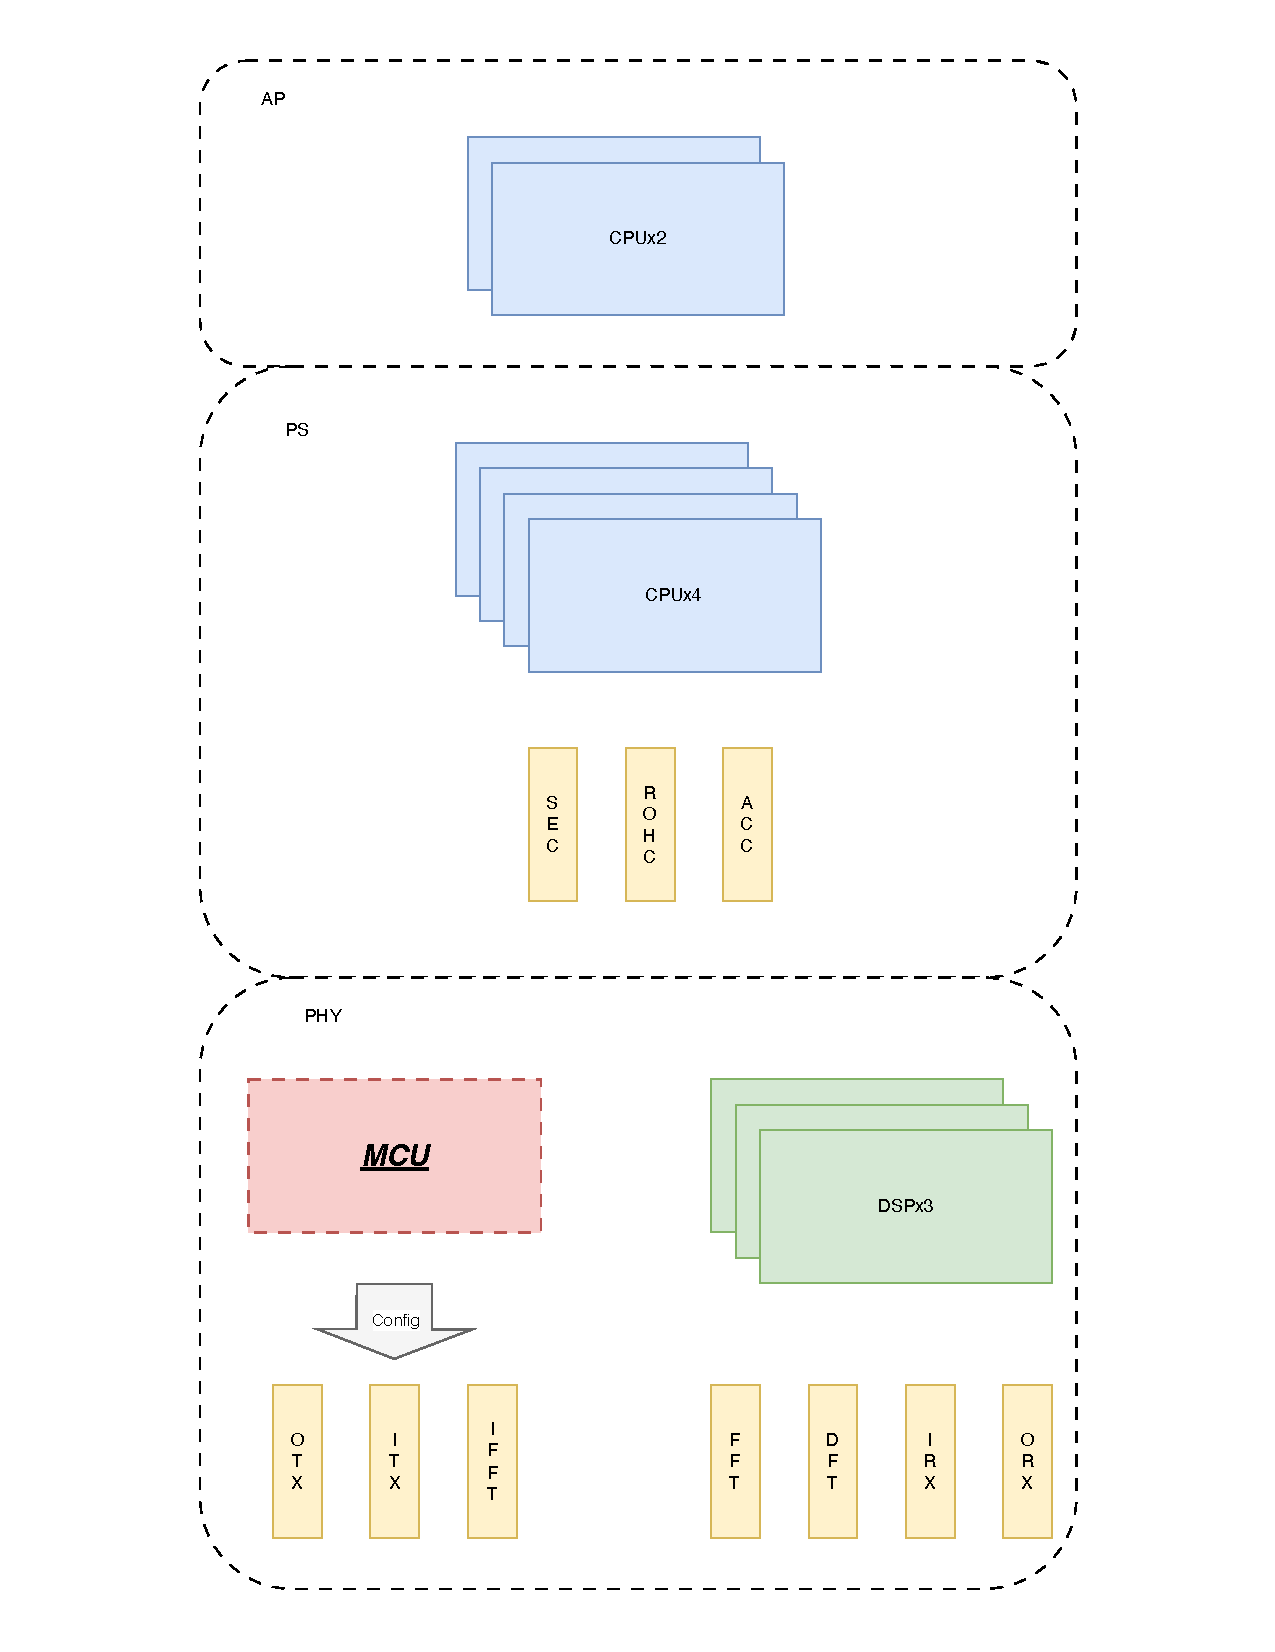
\includegraphics[scale=0.25]{./images/mcu_location.pdf}
  \caption{所设计微控制器在5G基带芯片中的位置}
  \label{fig:pic1}
\end{figure}

\newpage
\section{研究内容及当前进度}%
本课题主要目标是基于RISC-V指令集开发MCU,用于控制5G基带芯片内部的加速器。
需要满足快速响应及低功耗的特征。本课题的研究内容主要有三个方面,如图\ref{fig:research_topics}所示。
\begin{figure}[ht]
  \centering
  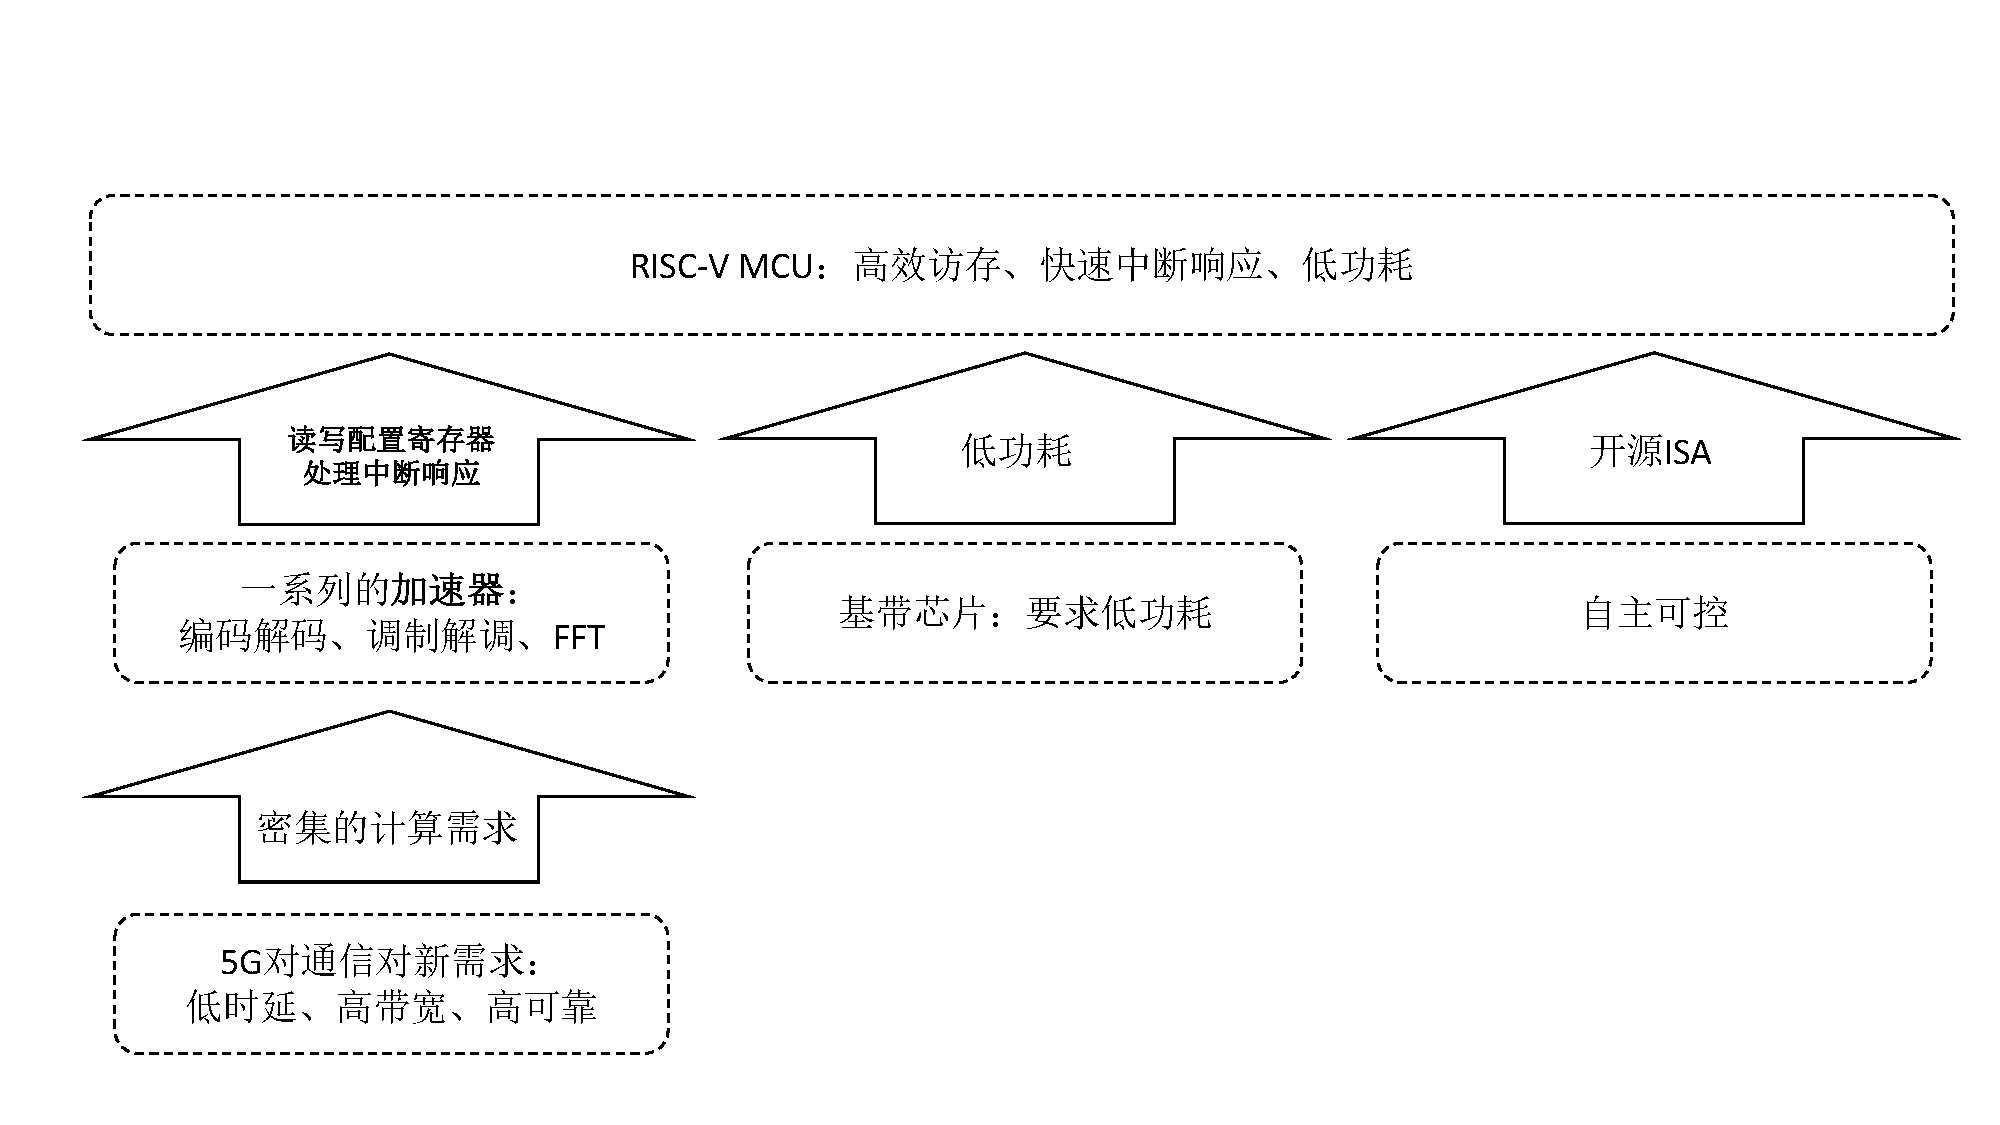
\includegraphics[width=0.8\linewidth]{./images/research_topics.pdf}
  \caption{本课题研究内容}
  \label{fig:research_topics}
\end{figure}

目前本课题主要研究内容及进度如表\ref{tab:tab1}所示
\begin{center}
\begin{tabular}{ c c c }
  \label{tab:tab1}
 cell1 & cell2 & cell3 \\ 
 cell4 & cell5 & cell6 \\  
 cell7 & cell8 & cell9    
\end{tabular}
\end{center}

\newpage
\section{已完成内容}%
\subsection{技术路线}%
本课题的技术路线采用\textbf{先实现再优化}的思想。首先根据当前项目的资料分析了需要解决的问题;确定加速器调度问题的主要应用场景之后确定了微控制器的主要任务,并且在此基础上确定了微控制器采用顺序单发射架构、支持RISC-V 32IMC指令集,其中乘法指令集(M)是为了保证微控制器一定的计算性能、压缩指令集(C)则是压缩程序所占用的存储面积,保证应用程序能够存储。

微控制器功能特性确定之后,按照五级流水线架构对微处理器进行了实现,其中模块集级验证采用了testbench进行简单验证;微控制器系统级验证采用了Difftest框架进行验证,验证通过了所有的RISC-V TESTS测试集,在一定程度上保证了微控制器是正确实现了RISC-V手册规范的。

在处理器核功能正确的基础上,针对加速器调度的场景以及低功耗需求进行了优化设计,主要特现在:取指部分针对整数指令地址不对齐做了优化;译码部分实现了分支预测器以及地址重定向的仲裁;访存部分针对加速器配置信息下发做了优化。优化设计完成之后对微控制器再次进行Difftest测试,保证微控制器优化设计之后依然符合RISC-V手册规范、检查优化之后的微控制器设计是否取得了设计的性能提升。
% 最后,将微控制器集成到5G基带芯片内做功能测试,对微控制器的功能跟性能进行测试。
  
\newpage
\subsection{研究方法}%
当前本课题已经实现了取指部分以及译码部分优化设计,针对访存部分的设计优化正在进行当中。
\subsubsection{取指部分}
\textbf{(a)问题提出}:由于5G基带芯片对于实时性的要求很高,因此用于加速器调度的微控制器本身也需要满足实时性的设计。在这个前提下,微控制器不能使用Cache做指令存储,因为Cache会存在Cache Miss的问题,导致取指部分的时延不能保证,违反了实时性的要求,因此取指部分采用\textbf{ITCM}(Instruction Tightly Coupuled Memory)做指令存储。
ITCM由于需要匹配微控制器的速度,其容量不能做到很大,因此在设计微控制器架构的时候需要实现压缩指令集,RISC-V手册规定其压缩指令(16 bits)跟整数指令(32 bit)在指令存储内部是混合存储的,因此引出了\textbf{整数指令跟压缩指令混合存储时整数指令的取指问题},该问题具体表现为如下两点:
\begin{enumerate}
  \item 当整数指令取指地址不是2B对齐的时候,如何访问一次ITCM在一个cycle内完成整数指令的取指。
  \item 整数指令跟压缩指令在指令存储内混合存放,微控制器如何对从指令存储内取出的指令做边界判定,识别出每一条压缩指令跟整数指令。
\end{enumerate}

\textbf{(b)研究目标}:微控制器的取指部分需要实现在一个cycle内取出一条整数指令,并且完成整数指令跟压缩指令的识别并且在整数指令地址不对齐的时候完成对整数指令的拼接。

\textbf{(c)设计方案}:取指部分采用\textbf{odd even ITCM 跟取指FIFO}来实现上述的设计目标。其设计目标如图\ref{fig:if_design_features}所示。
\begin{figure}
  \centering
  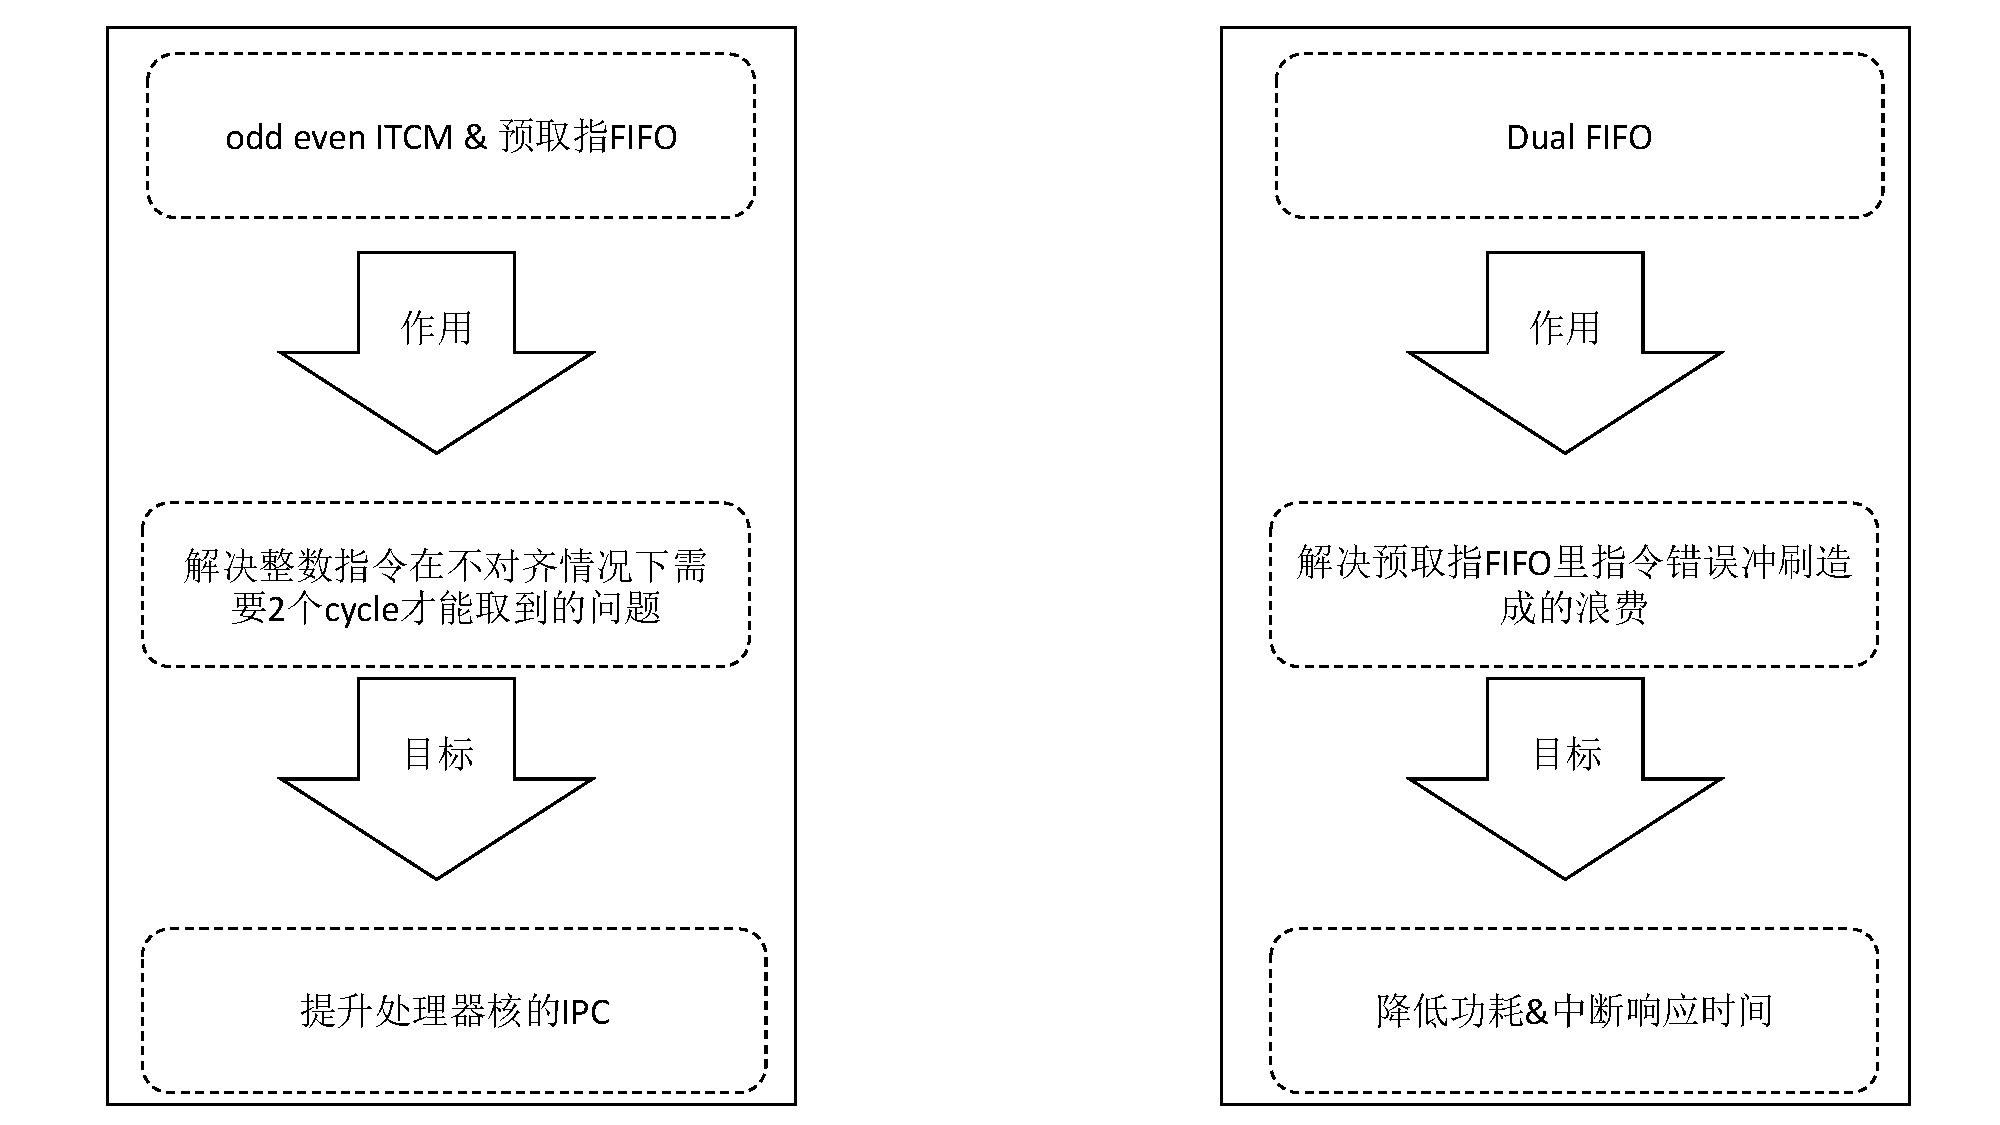
\includegraphics[width=0.8\linewidth]{./images/if_design_features.pdf}
  \caption{采用odd even ITCM跟取指FIFO解决整数指令跟压缩指令混合存储时整数指令取指问题}
  \label{fig:if_design_features}
\end{figure}

\begin{itemize}
  \item \textbf{odd even ITCM}:
    指令的取指地址可能是4B对齐也可能是2B对齐的,地址2B对齐的时候需要访问两次ITCM才可以才可以从ITCM里取出整数指令的高16bits跟低16bits,再通过拼接电路完成整数指令的拼接。\\ 
    当地址是连续递增的时候可以采用\textit{leftover buffer}存储上一次访问ITCM得到的高16 bits数据,如图\ref{fig:if_leftover_buffer}所示。当地址2B对齐的时候可以利用\textit{leftover buffer}里的内容实现整数指令的拼接。\textit{但是这种方法在地址出现跳转时会失效}。
    \begin{figure}[ht]
      \centering
      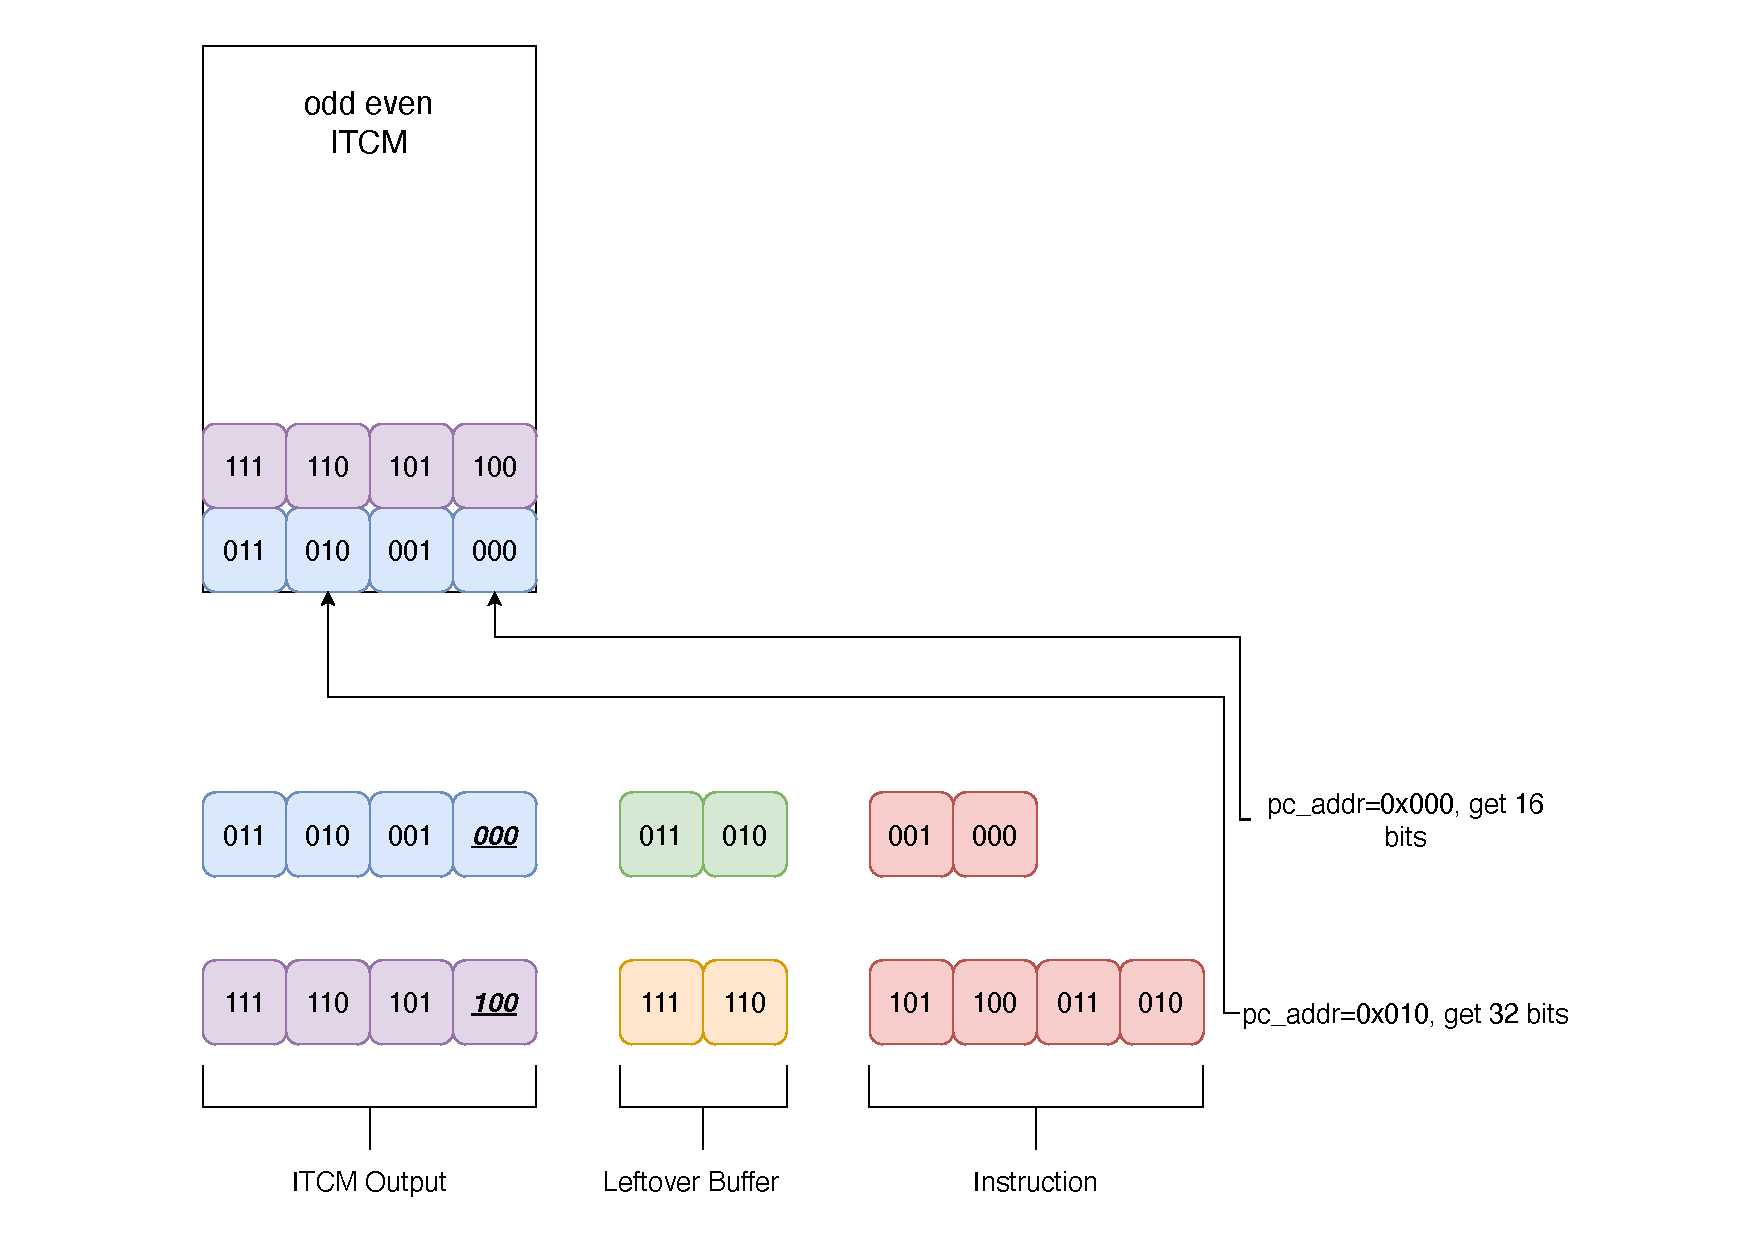
\includegraphics[width=0.8\linewidth]{./images/if_leftover_buffer.pdf}
      \caption{采用leftover buffer来实现整数指令的拼接}
      \label{fig:if_leftover_buffer}
    \end{figure}
    本课题采用\textit{odd even ITCM}可以解决指令跳转后出现地址不是4B对齐时的整数指令的取指问题。其核心思想在于\textbf{将ITCM分为odd, even}两部分,两部分可以独立的访问。当地址不是4B对齐的时候,\textit{even ITCM}访问地址比\textit{odd ITCM}高一位,并且将\textit{even ITCM}里的数据当作高16 bits,\textit{odd ITCM}里的数据当低16 bits完成指令的拼接;当地址是4B对齐的时候,两块ITCM的访问地址一样,并且\textit{even ITCM}的数据当作低16 bits完成指令的拼接。具体操作原理如图TBD所示。
  \item \textbf{取指FIFO}
    在访问ITCM的时候,只能根据地址是否是4B对齐控制访问ITCM的动作,但是从ITCM里取出的指令可能的组合有如下五种情况TBD 增加论文ref:
    \begin{enumerate}
      \item 取出的32 bits数据是一条整数指令
      \item 取出的32 bits数据是两条压缩指令
      \item 取出的32 bits数据是一条压缩指令跟一条整数指令的低16 bits
      \item 取出的32 bits数据是一条整数指令高16 bits跟一条压缩指令
      \item 取出的32 bits数据是一条整数指令高16 bits跟一条整数指令低16 bits
    \end{enumerate}
为了判断具体指令的类型,需要复杂的硬件电路来从上述五种可能的情况里判断出取出的数据具体属于哪种类型,然后根据当前指令的类型来更新下一次取指地址的值。这会导致如下的缺陷:
\begin{enumerate}
  \item 取指级的周期变长:取出来的数据需要复杂的硬件电路才可以判断出指令的类型,这会增减组合逻辑电路的延时;下一次取指的地址需要根据当前指令的类型选择加4或者加2。
  \item 在可能的组合2、4中,高16 bits的压缩指令会被重复取出,因为这两种情况下取指地址会加2,导致了额外的访存功耗。
\end{enumerate}
基于上述硬件电路的缺点,本课题提出了\textit{5*16}的取指FIFO,用于存储从ITCM中取出的数据、完成指令类型的判断以及整数指令的拼接,其结构如图TBD所示;其操作逻辑如下:
\begin{enumerate}
  \item FIFO总容量为5,表示其内部的5个16 bits的寄存器。容量设计为5是为了避免写入到FIFO的时候出现overflow。
  \item 从ITCM中每次都会得到32 bits的数据,当FIFO容量$\le 3$的时候FIFO允许被写入,取出的32 bits数据会被push到FIFO中。
  \item 当译码级没有被stall的时候,每个cycle会译码一条指令,译码的时候会判断FIFO头部寄存器的低2 bits是否是\textit{11}。根据RISC-V规定,指令低2 bits如果是11则表示当前指令是一条整数指令,此时会从FIFO头部pop出2个16bits的数据,即一条整数指令;反之如果低2 bits不是11,则说明当前指令是一条压缩指令,此时只需要pop出FIFO头部一条指令即可。
\end{enumerate}
  \item \textbf{Dual FIFO}
\end{itemize}


\subsubsection{译码部分}
  

\newpage
\section{未来工作计划}%



% \newpage
% \bibliography{ref} % 参考文献源,存储所有的参考文献
% \bibliographystyle{IEEEtran} % latex饮用参考文献时的格式
\end{document}

